\subsection{Quelques notations et résultats}

\subsubsection{Résumé des notations}

Résumons ici quelques notations utiles pour la suite, de manière informelle :

\begin{itemize}
\item Valeurs de vérité : $\mathrm{V}$ (« vrai »), $\mathrm{I}$ (« indéfini »), $\mathrm{F}$ (« faux »).
\item Le symbole $\neg$ représente la négation : si $P$ est une proposition, la proposition $\neg P$ est fausse si $P$ est vraie et inversement. 
    Sa table de vérité est donnée ci-dessous : 
\begin{center}
\begin{tabular}{c | c}
    $P$ & $\neg P$ \\
    \hline
    $\mathsf{V}$ & $\mathsf{F}$ \\
    $\mathsf{I}$ & $\mathsf{I}$ \\
    $\mathsf{F}$ & $\mathsf{V}$ \\
\end{tabular} .
\end{center}
\item Les symboles $\wedge$ et $\vee$ représentent respectivement les connecteurs « et » et « ou ». 
Les symboles $\Rightarrow$ et $\Leftarrow$ représentent l'implication vers la droite et vers la gauche. 
Le symbole $\Leftrightarrow$ représente l'équivalence. 
    Soit $P$ et $Q$ deux propositions, on a ainsi la table de vérité suivante : 
\begin{center}
\begin{tabular}{c c | c c c c c}
    $P$ & $Q$ & $P \wedge Q$ & $P \vee Q$ & $P \Rightarrow Q$ & $P \Leftarrow Q$ & $P \Leftrightarrow Q$ \\
    \hline
    $\mathsf{V}$ & $\mathsf{V}$ & $\mathsf{V}$ & $\mathsf{V}$ & $\mathsf{V}$ & $\mathsf{V}$ & $\mathsf{V}$ \\
    $\mathsf{V}$ & $\mathsf{I}$ & $\mathsf{I}$ & $\mathsf{V}$ & $\mathsf{I}$ & $\mathsf{V}$ & $\mathsf{I}$ \\
    $\mathsf{V}$ & $\mathsf{F}$ & $\mathsf{F}$ & $\mathsf{V}$ & $\mathsf{F}$ & $\mathsf{V}$ & $\mathsf{F}$ \\
    $\mathsf{I}$ & $\mathsf{V}$ & $\mathsf{I}$ & $\mathsf{V}$ & $\mathsf{V}$ & $\mathsf{I}$ & $\mathsf{I}$ \\
    $\mathsf{I}$ & $\mathsf{I}$ & $\mathsf{I}$ & $\mathsf{I}$ & $\mathsf{I}$ & $\mathsf{I}$ & $\mathsf{I}$ \\
    $\mathsf{I}$ & $\mathsf{F}$ & $\mathsf{F}$ & $\mathsf{I}$ & $\mathsf{I}$ & $\mathsf{V}$ & $\mathsf{I}$ \\
    $\mathsf{F}$ & $\mathsf{V}$ & $\mathsf{F}$ & $\mathsf{V}$ & $\mathsf{V}$ & $\mathsf{F}$ & $\mathsf{F}$ \\
    $\mathsf{F}$ & $\mathsf{I}$ & $\mathsf{F}$ & $\mathsf{I}$ & $\mathsf{V}$ & $\mathsf{I}$ & $\mathsf{I}$ \\
    $\mathsf{F}$ & $\mathsf{F}$ & $\mathsf{F}$ & $\mathsf{F}$ & $\mathsf{V}$ & $\mathsf{V}$ & $\mathsf{V}$ \\
\end{tabular} .
\end{center}
\item Les symboles $\forall$ et $\exists$ représentent respectivement les quantificateurs universel (« pour tout ») et existentiel (« il existe »). 
\item On note $\in$ la relation d'appartenance et $\notin$ sa négation : $\forall x \forall y \, x \notin y \Leftrightarrow \not (x _in y)$.
\item L'ensemble vide est noté $\emptyset$.
\item Soit $a$ un ensemble. 
    On note $\lbrace a \rbrace$ l'ensemble contenant uniquement $a$. 
\item Soit $a$ et $b$ deux ensembles.
    On note $\lbrace a, b \rbrace$ la paire de $a$ et $b$, \textit{i.e.} l'ensemble définit par : 
\begin{equation*}
    \forall x \, x \in \lbrace a, b \rbrace \Leftrightarrow ((x = a) \wedge (x = b))
\end{equation*}
\item Soit $E$ un ensemble et $P$ un prédicat à un paramètre libre. 
    L'ensemble $\lbrace x \in E \vert P x \rbrace$ (noté $F$ dans la formule ci-dessous) est le sous-ensemble de $E$ défini par : 
\begin{equation*}
    \forall x \, x \in F \Leftrightarrow x \in E \wedge P x. 
\end{equation*}
    On note $(a,b)$ le couple formé par $a$ et $b$, définit par : $(a,b) = \lbrace \lbrace a \rbrace, \lbrace a, b \rbrace \rbrace$.
\item Soit $E$ et $F$ deux ensembles. 
L'\textit{union} de $E$ et $F$, notée $E \cup F$, est l'ensemble défini par : 
\begin{equation*}
    E \cup F = \lbrace x \vert (x \in E) \vee (x \in F)  \rbrace . 
\end{equation*}
L'\textit{intersection} de $E$ et $F$, notée $E \cap F$, est l'ensemble défini par :
\begin{equation*}
    E \cap F = \lbrace x \vert (x \in E) \wedge (x \in F)  \rbrace. 
\end{equation*}
La \textit{différence} de $E$ et $F$, notée $E \setminus F$, est l'ensemble défini par :
\begin{equation*}
    E \setminus F = \lbrace x \vert (x \in E) \wedge (x \notin F)  \rbrace. 
\end{equation*}
\item Soit $E$ et $F$ deux ensembles.
On dit que $E$ est inclus dans $F$, et on note $E \subset F$ ou $F \supset E$, si la proposition suivante est vraie : $\forall \, x \, x \in E \Rightarrow x \in F$. 
\end{itemize}

\subsubsection{Ensemble de tous les ensembles} 

\noindent\textbf{Lemme :} Il n'existe pas d'ensemble de tous les ensembles. 

\medskip

\noindent\textbf{Démonstration :} Supposons par l'absurde que l'ensemble de tous les ensembles existe, et notons-le $U$. 
Définissons l'ensemble $X$ par : $X = \lbrace e \in U \vert e \notin e \rbrace$%
~\footnote{
    Cet ensemble existe d'après le schéma d'axiomes de compréhensions. 
    En ré-utilisant les notations de l'énoncé de cet axiomes, il s'agit de l'ensemble obtenu en prenant $a = U$ et $P x: x \notin x$.
}%
, et considérons la propriété $P: X \in X$. 
Alors, 
\begin{itemize}[nosep]
    \item Si $P$ est vraie, $X \in X$, donc, par définition de cet ensemble, $X$ n'est pas un élément de $X$, et donc $P$ est fausse. 
    \item Si $P$ est fausse, $X \notin X$, donc, par définition de cet ensemble, $X$ est un élément de $X$, et donc $P$ est vraie. 
\end{itemize}
Ainsi, la propriété $P$ ne peut être ni vraie ni fausse, ce qui constitue une contradiction. 
On en déduit que l'hypothèse de départ est fausse. 

\hfill\square

\medskip

\noindent\textbf{NB:} Si on inclus la valeur de vérite « indéfinie » dans la théorie, alors cette démonstration montre seulement que, avec les mêmes notations, la propriété $P$ est indéfinie.

\medskip

\noindent\textbf{NB:} Le résultat est évident si l'on inclus l'axiome de fondation dans la théorie, puisqu'alors aucun ensemble ne peut être élément de lui-même.


\subsubsection{Représentations schématiques}

Nous donnons ici des représentations schématiques de certains des concepts définis ci-dessus. 
Ces schémas sont destinés à donner une représentation intuitive de ces concepts, et n'ont aucunement prétention à aucune forme de rigueur.

\bigskip
\bigskip

\begin{minipage}{\linewidth}
\centering
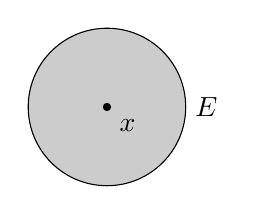
\begin{tikzpicture}
    \draw[fill=black, fill opacity=0.2] (0,0) circle (1cm);
    \node[right] at (1cm,0) {$E$};
    \node[circle, fill, minimum size=3pt, inner sep=0pt, outer sep=0pt, label=below right:$x$] at (0,0) {};
\end{tikzpicture}

$x \in E$
\end{minipage}

\bigskip
\bigskip

\begin{minipage}{\linewidth}
\centering
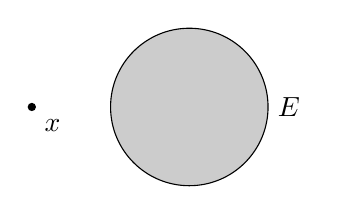
\begin{tikzpicture}
    \draw[fill=black, fill opacity=0.2] (0,0) circle (1cm);
    \node[right] at (1cm,0) {$E$};
    \node[circle, fill, minimum size=3pt, inner sep=0pt, outer sep=0pt, label=below right:$x$] at (-2cm,0) {};
\end{tikzpicture}

$x \notin E$
\end{minipage}

\bigskip
\bigskip

\begin{minipage}{\linewidth}
\centering
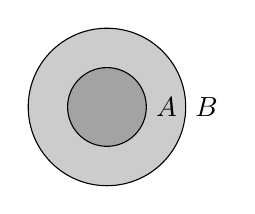
\begin{tikzpicture}
    \draw[fill=black, fill opacity=0.2] (0,0) circle (1cm);
    \draw[fill=black, fill opacity=0.2] (0,0) circle (0.5cm);
    \node[right] at (0.5cm,0) {$A$};
    \node[right] at (1cm,0) {$B$};
\end{tikzpicture}

$A \subset B$
\end{minipage}

\bigskip
\bigskip

Sur chacun des quatre schémas suivants, la zone grisée correspond à l'ensemble en légende.

\bigskip
\bigskip

\begin{minipage}{\linewidth}
\centering
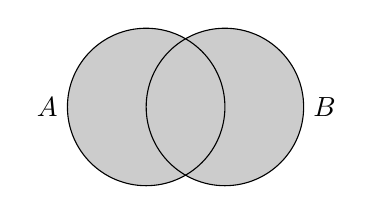
\begin{tikzpicture}
    \fill[black!20!white] (0.5cm,0) circle (1cm);
    \fill[black!20!white] (-0.5cm,0) circle (1cm);
    \draw (0.5cm,0) circle (1cm);
    \draw (-0.5cm,0) circle (1cm);
    \node[left] at (-1.5cm,0) {$A$};
    \node[right] at (1.5cm,0) {$B$};
\end{tikzpicture}

$A \cup B$
\end{minipage}

\bigskip
\bigskip

\begin{minipage}{\linewidth}
\centering
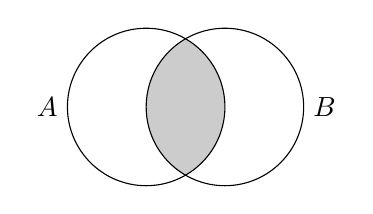
\begin{tikzpicture}
    \begin{scope}
        \clip (0.5cm,0) circle(1cm);
        \fill[black!20!white] (-0.5cm,0) circle (1cm);
    \end{scope}
    \draw (0.5cm,0) circle (1cm);
    \draw (-0.5cm,0) circle (1cm);
    \node[left] at (-1.5cm,0) {$A$};
    \node[right] at (1.5cm,0) {$B$};
\end{tikzpicture}

$A \cap B$
\end{minipage}

\bigskip
\bigskip

\begin{minipage}{\linewidth}
\centering
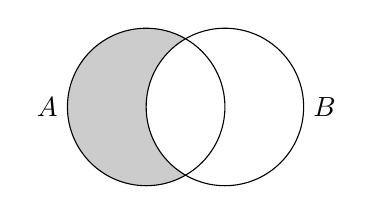
\begin{tikzpicture}
    \fill[black!20!white] (-0.5cm,0) circle (1cm);
    \begin{scope}
        \clip (0.5cm,0) circle(1cm);
        \fill[white] (-0.5cm,0) circle (1cm);
    \end{scope}
    \draw (0.5cm,0) circle (1cm);
    \draw (-0.5cm,0) circle (1cm);
    \node[left] at (-1.5cm,0) {$A$};
    \node[right] at (1.5cm,0) {$B$};
\end{tikzpicture}

$A \setminus B$
\end{minipage}

\bigskip
\bigskip

\begin{minipage}{\linewidth}
\centering
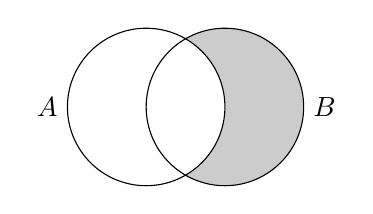
\begin{tikzpicture}
    \fill[black!20!white] (0.5cm,0) circle (1cm);
    \begin{scope}
        \clip (0.5cm,0) circle(1cm);
        \fill[white] (-0.5cm,0) circle (1cm);
    \end{scope}
    \draw (0.5cm,0) circle (1cm);
    \draw (-0.5cm,0) circle (1cm);
    \node[left] at (-1.5cm,0) {$A$};
    \node[right] at (1.5cm,0) {$B$};
\end{tikzpicture}

$B \setminus A$
\end{minipage}

\bigskip
\bigskip

Certains résultats se voient aisément schématiquement : 

\bigskip
\bigskip

\begin{minipage}{\linewidth}
\centering
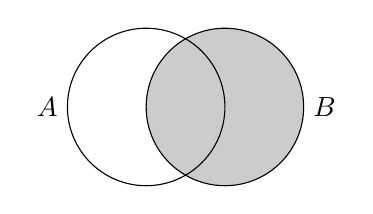
\begin{tikzpicture}
    \fill[white] (-0.5cm,0) circle (1cm);
    \fill[black!20!white] (0.5cm,0) circle (1cm);
    \draw (0.5cm,0) circle (1cm);
    \draw (-0.5cm,0) circle (1cm);
    \node[left] at (-1.5cm,0) {$A$};
    \node[right] at (1.5cm,0) {$B$};
\end{tikzpicture}

$(B \setminus A) \cup (A \cap B) = B$
\end{minipage}

\bigskip
\bigskip

\begin{minipage}{\linewidth}
\centering
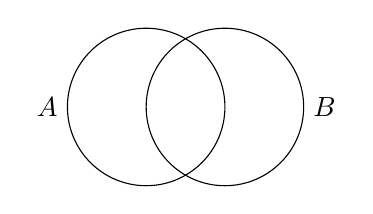
\begin{tikzpicture}
    \fill[white] (-0.5cm,0) circle (1cm);
    \fill[white] (0.5cm,0) circle (1cm);
    \draw (0.5cm,0) circle (1cm);
    \draw (-0.5cm,0) circle (1cm);
    \node[left] at (-1.5cm,0) {$A$};
    \node[right] at (1.5cm,0) {$B$};
\end{tikzpicture}

$(B \setminus A) \cap (A \cap B) = \emptyset$
\end{minipage}

\bigskip
\bigskip

\begin{minipage}{\linewidth}
\centering
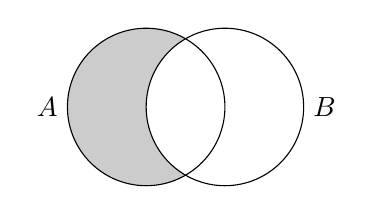
\begin{tikzpicture}
    \fill[black!20!white] (-0.5cm,0) circle (1cm);
    \fill[white] (0.5cm,0) circle (1cm);
    \draw (0.5cm,0) circle (1cm);
    \draw (-0.5cm,0) circle (1cm);
    \node[left] at (-1.5cm,0) {$A$};
    \node[right] at (1.5cm,0) {$B$};
\end{tikzpicture}

$(A \cup B) \setminus B = A \setminus B$
\end{minipage}

\bigskip
\bigskip

Une fonction d'un ensemble $E$ vers un ensemble $F$ peut être représentée par des flèches allant de chaque élément de $E$ vers son image. 

\bigskip
\bigskip

\begin{minipage}{\linewidth}
\centering
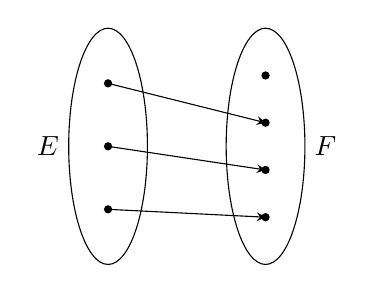
\begin{tikzpicture}
    \draw (-1cm,0) ellipse (0.5cm and 1.5cm);
    \draw (1cm,0) ellipse (0.5cm and 1.5cm);
    \node[left] at (-1.5cm,0) {$E$};
    \node[right] at (1.5cm,0) {$F$};
    \node[fill, circle, minimum size=3pt, inner sep=0, outer sep=0] at (-1cm,0.8cm) {};
    \node[fill, circle, minimum size=3pt, inner sep=0, outer sep=0] at (-1cm,0) {};
    \node[fill, circle, minimum size=3pt, inner sep=0, outer sep=0] at (-1cm,-0.8cm) {};
    \node[fill, circle, minimum size=3pt, inner sep=0, outer sep=0] at (1cm,0.9cm) {};
    \node[fill, circle, minimum size=3pt, inner sep=0, outer sep=0] at (1cm,0.3cm) {};
    \node[fill, circle, minimum size=3pt, inner sep=0, outer sep=0] at (1cm,-0.3cm) {};
    \node[fill, circle, minimum size=3pt, inner sep=0, outer sep=0] at (1cm,-0.9cm) {};
    \draw[-stealth] (-1cm,0.8cm) -- (1cm, 0.3cm);
    \draw[-stealth] (-1cm,0) -- (1cm, -0.3cm);
    \draw[-stealth] (-1cm,-0.8cm) -- (1cm, -0.9cm);
\end{tikzpicture}

Exemple d'injection
\end{minipage}

\bigskip
\bigskip

\begin{minipage}{\linewidth}
\centering
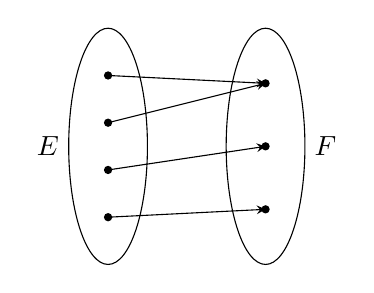
\begin{tikzpicture}
    \draw (-1cm,0) ellipse (0.5cm and 1.5cm);
    \draw (1cm,0) ellipse (0.5cm and 1.5cm);
    \node[left] at (-1.5cm,0) {$E$};
    \node[right] at (1.5cm,0) {$F$};
    \node[fill, circle, minimum size=3pt, inner sep=0, outer sep=0] at (-1cm,0.9cm) {};
    \node[fill, circle, minimum size=3pt, inner sep=0, outer sep=0] at (-1cm,0.3cm) {};
    \node[fill, circle, minimum size=3pt, inner sep=0, outer sep=0] at (-1cm,-0.3cm) {};
    \node[fill, circle, minimum size=3pt, inner sep=0, outer sep=0] at (-1cm,-0.9cm) {};
    \node[fill, circle, minimum size=3pt, inner sep=0, outer sep=0] at (1cm,0.8cm) {};
    \node[fill, circle, minimum size=3pt, inner sep=0, outer sep=0] at (1cm,0) {};
    \node[fill, circle, minimum size=3pt, inner sep=0, outer sep=0] at (1cm,-0.8cm) {};
    \draw[-stealth] (-1cm,0.9cm) -- (1cm, 0.8cm);
    \draw[-stealth] (-1cm,0.3cm) -- (1cm, 0.8cm);
    \draw[-stealth] (-1cm,-0.3cm) -- (1cm, 0);
    \draw[-stealth] (-1cm,-0.9cm) -- (1cm, -0.8cm);
\end{tikzpicture}

Exemple de surjection
\end{minipage}

\bigskip
\bigskip

\begin{minipage}{\linewidth}
\centering
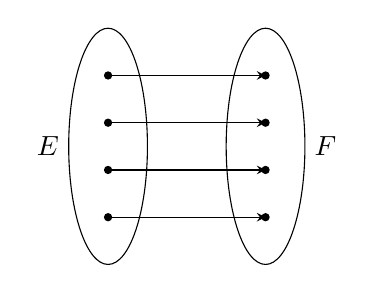
\begin{tikzpicture}
    \draw (-1cm,0) ellipse (0.5cm and 1.5cm);
    \draw (1cm,0) ellipse (0.5cm and 1.5cm);
    \node[left] at (-1.5cm,0) {$E$};
    \node[right] at (1.5cm,0) {$F$};
    \node[fill, circle, minimum size=3pt, inner sep=0, outer sep=0] at (-1cm,0.9cm) {};
    \node[fill, circle, minimum size=3pt, inner sep=0, outer sep=0] at (-1cm,0.3cm) {};
    \node[fill, circle, minimum size=3pt, inner sep=0, outer sep=0] at (-1cm,-0.3cm) {};
    \node[fill, circle, minimum size=3pt, inner sep=0, outer sep=0] at (-1cm,-0.9cm) {};
    \node[fill, circle, minimum size=3pt, inner sep=0, outer sep=0] at (1cm,0.9cm) {};
    \node[fill, circle, minimum size=3pt, inner sep=0, outer sep=0] at (1cm,0.3cm) {};
    \node[fill, circle, minimum size=3pt, inner sep=0, outer sep=0] at (1cm,-0.3cm) {};
    \node[fill, circle, minimum size=3pt, inner sep=0, outer sep=0] at (1cm,-0.9cm) {};
    \draw[-stealth] (-1cm,0.9cm) -- (1cm, 0.9cm);
    \draw[-stealth] (-1cm,0.3cm) -- (1cm, 0.3cm);
    \draw[-stealth] (-1cm,-0.3cm) -- (1cm, -0.3cm);
    \draw[-stealth] (-1cm,-0.9cm) -- (1cm, -0.9cm);
\end{tikzpicture}

Exemple de bijection
\end{minipage}

\bigskip
\bigskip

\begin{minipage}{\linewidth}
\centering
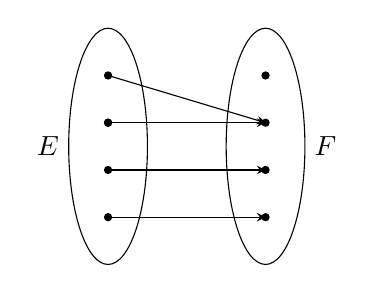
\begin{tikzpicture}
    \draw (-1cm,0) ellipse (0.5cm and 1.5cm);
    \draw (1cm,0) ellipse (0.5cm and 1.5cm);
    \node[left] at (-1.5cm,0) {$E$};
    \node[right] at (1.5cm,0) {$F$};
    \node[fill, circle, minimum size=3pt, inner sep=0, outer sep=0] at (-1cm,0.9cm) {};
    \node[fill, circle, minimum size=3pt, inner sep=0, outer sep=0] at (-1cm,0.3cm) {};
    \node[fill, circle, minimum size=3pt, inner sep=0, outer sep=0] at (-1cm,0.3cm) {};
    \node[fill, circle, minimum size=3pt, inner sep=0, outer sep=0] at (-1cm,-0.3cm) {};
    \node[fill, circle, minimum size=3pt, inner sep=0, outer sep=0] at (-1cm,-0.9cm) {};
    \node[fill, circle, minimum size=3pt, inner sep=0, outer sep=0] at (1cm,0.9cm) {};
    \node[fill, circle, minimum size=3pt, inner sep=0, outer sep=0] at (1cm,0.3cm) {};
    \node[fill, circle, minimum size=3pt, inner sep=0, outer sep=0] at (1cm,-0.3cm) {};
    \node[fill, circle, minimum size=3pt, inner sep=0, outer sep=0] at (1cm,-0.9cm) {};
    \draw[-stealth] (-1cm,0.9cm) -- (1cm, 0.3cm);
    \draw[-stealth] (-1cm,0.3cm) -- (1cm, 0.3cm);
    \draw[-stealth] (-1cm,-0.3cm) -- (1cm, -0.3cm);
    \draw[-stealth] (-1cm,-0.9cm) -- (1cm, -0.9cm);
\end{tikzpicture}

Exemple de fonction ni injective ni bijective
\end{minipage}
